% 02 Challenges
\section{2. Identifying Challenges}

\subsection{2.1 Real-Time Data Acquisition from PX4}

The first significant challenge was establishing reliable real-time communication with the PX4 flight controller. PX4 uses the MAVLink protocol for all telemetry transmission, requiring a robust client implementation that could:

\begin{itemize}
    \item Handle multiple message types simultaneously
    \item Maintain connection stability during flight operations
    \item Log data at consistent rates without dropped packets
    \item Process various message formats (GPS, IMU, estimator status, etc.)
\end{itemize}

We implemented a custom MAVLink client using pymavlink that handles 8 message types: GLOBAL\_POSITION\_INT, GPS\_RAW\_INT, ATTITUDE, VIBRATION, ESTIMATOR\_STATUS, HEARTBEAT, SYS\_STATUS, and VFR\_HUD.

% Statistics box removed - can be added as text later
\textbf{Dataset Statistics:} 4,923 rows collected, 4,922 after cleaning, 504.6 seconds flight time at 10Hz sampling rate.
\vspace{0.5cm}

\subsection{2.2 Automated Labeling of Anomalies}

Without a physical GPS spoofer to generate labeled training data, we developed heuristic rules to identify anomalous GPS behavior based on:

\begin{itemize}
    \item GPS Monitor, Live Inference, Dashboard, PX4 simulation controls
    \item ML Pipeline buttons (Process, Train, Full)
    \item Kill Gazebo for simulation cleanup
    \item Data file information display
\end{itemize}

\begin{enumerate}
    \item Start/stop individual components independently
    \item Monitor component status in real-time
    \item Handle process lifecycle (PID management)
    \item Provide access to logs and output
    \item Start All / Stop All batch operations
    \item Train ML models
\end{enumerate}

\subsection{2.5 PX4 Simulation Environment}

We use PX4 Software-in-the-Loop (SITL) simulation with Gazebo for realistic testing:

\begin{itemize}
    \item Full PX4 flight stack execution
    \item Gazebo-based physics simulation (Iris x500 model)
    \item MAVLink communication on UDP port 14560
    \item Interactive pxh shell access
    \item Real-time telemetry output
\end{itemize}

\begin{figure}[htbp]
    \centering
    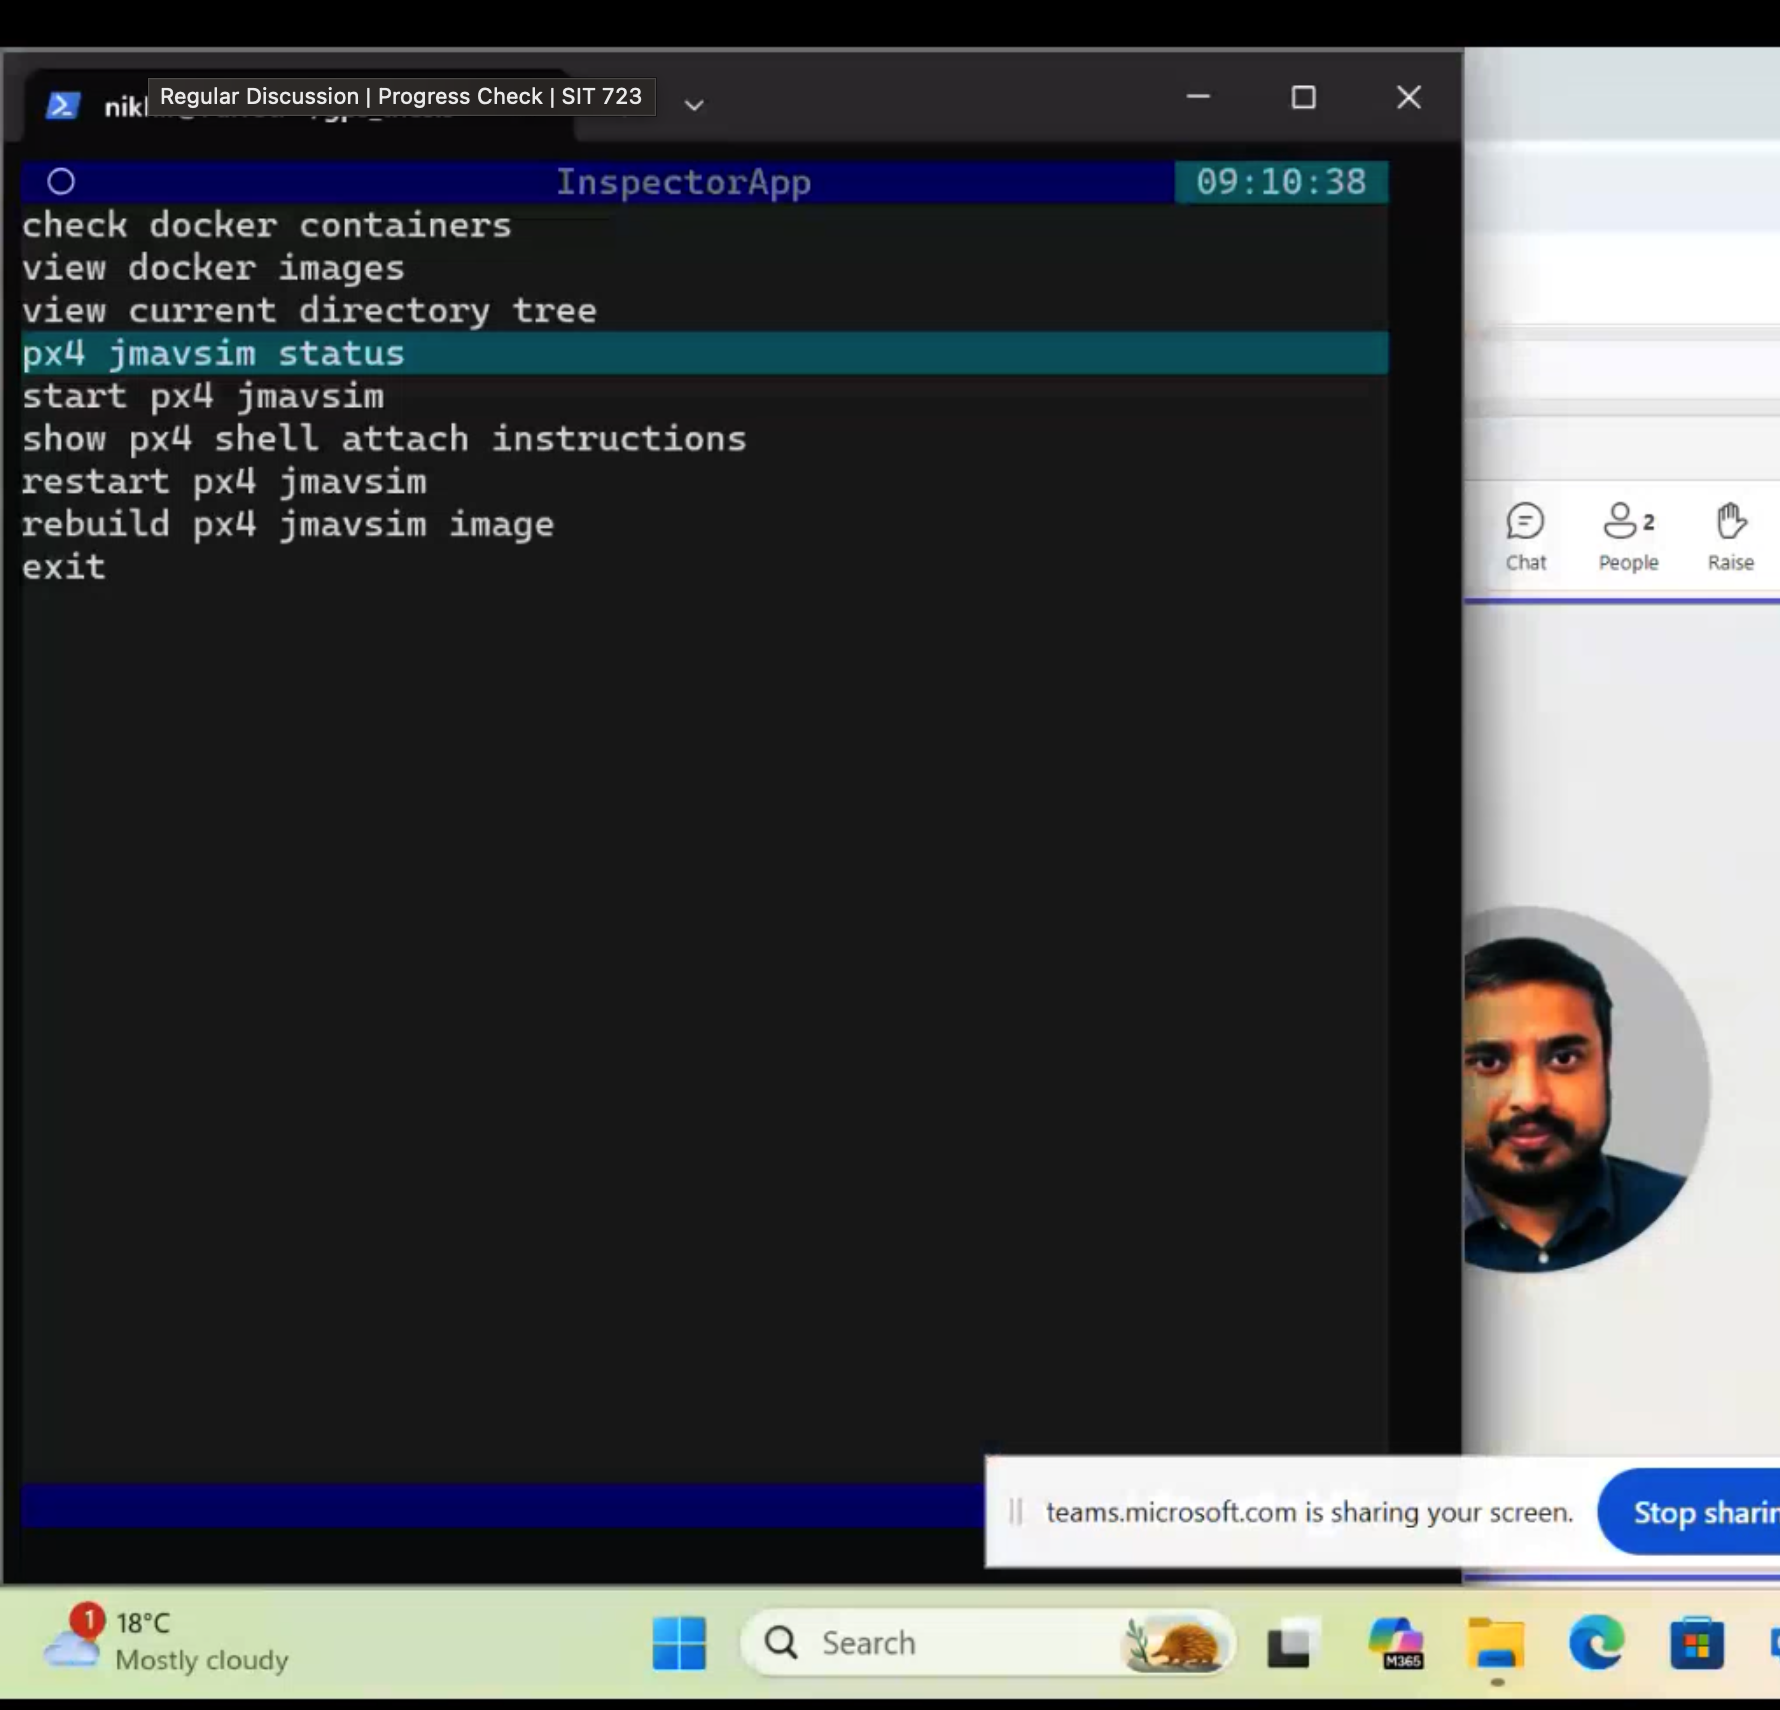
\includegraphics[width=0.7\linewidth]{figures/inspector tool created in second week.png}
    \caption{Terminal User Interface (Inspector Tool)}
    \label{fig:tui}
\end{figure}

\begin{figure}[htbp]
    \centering
    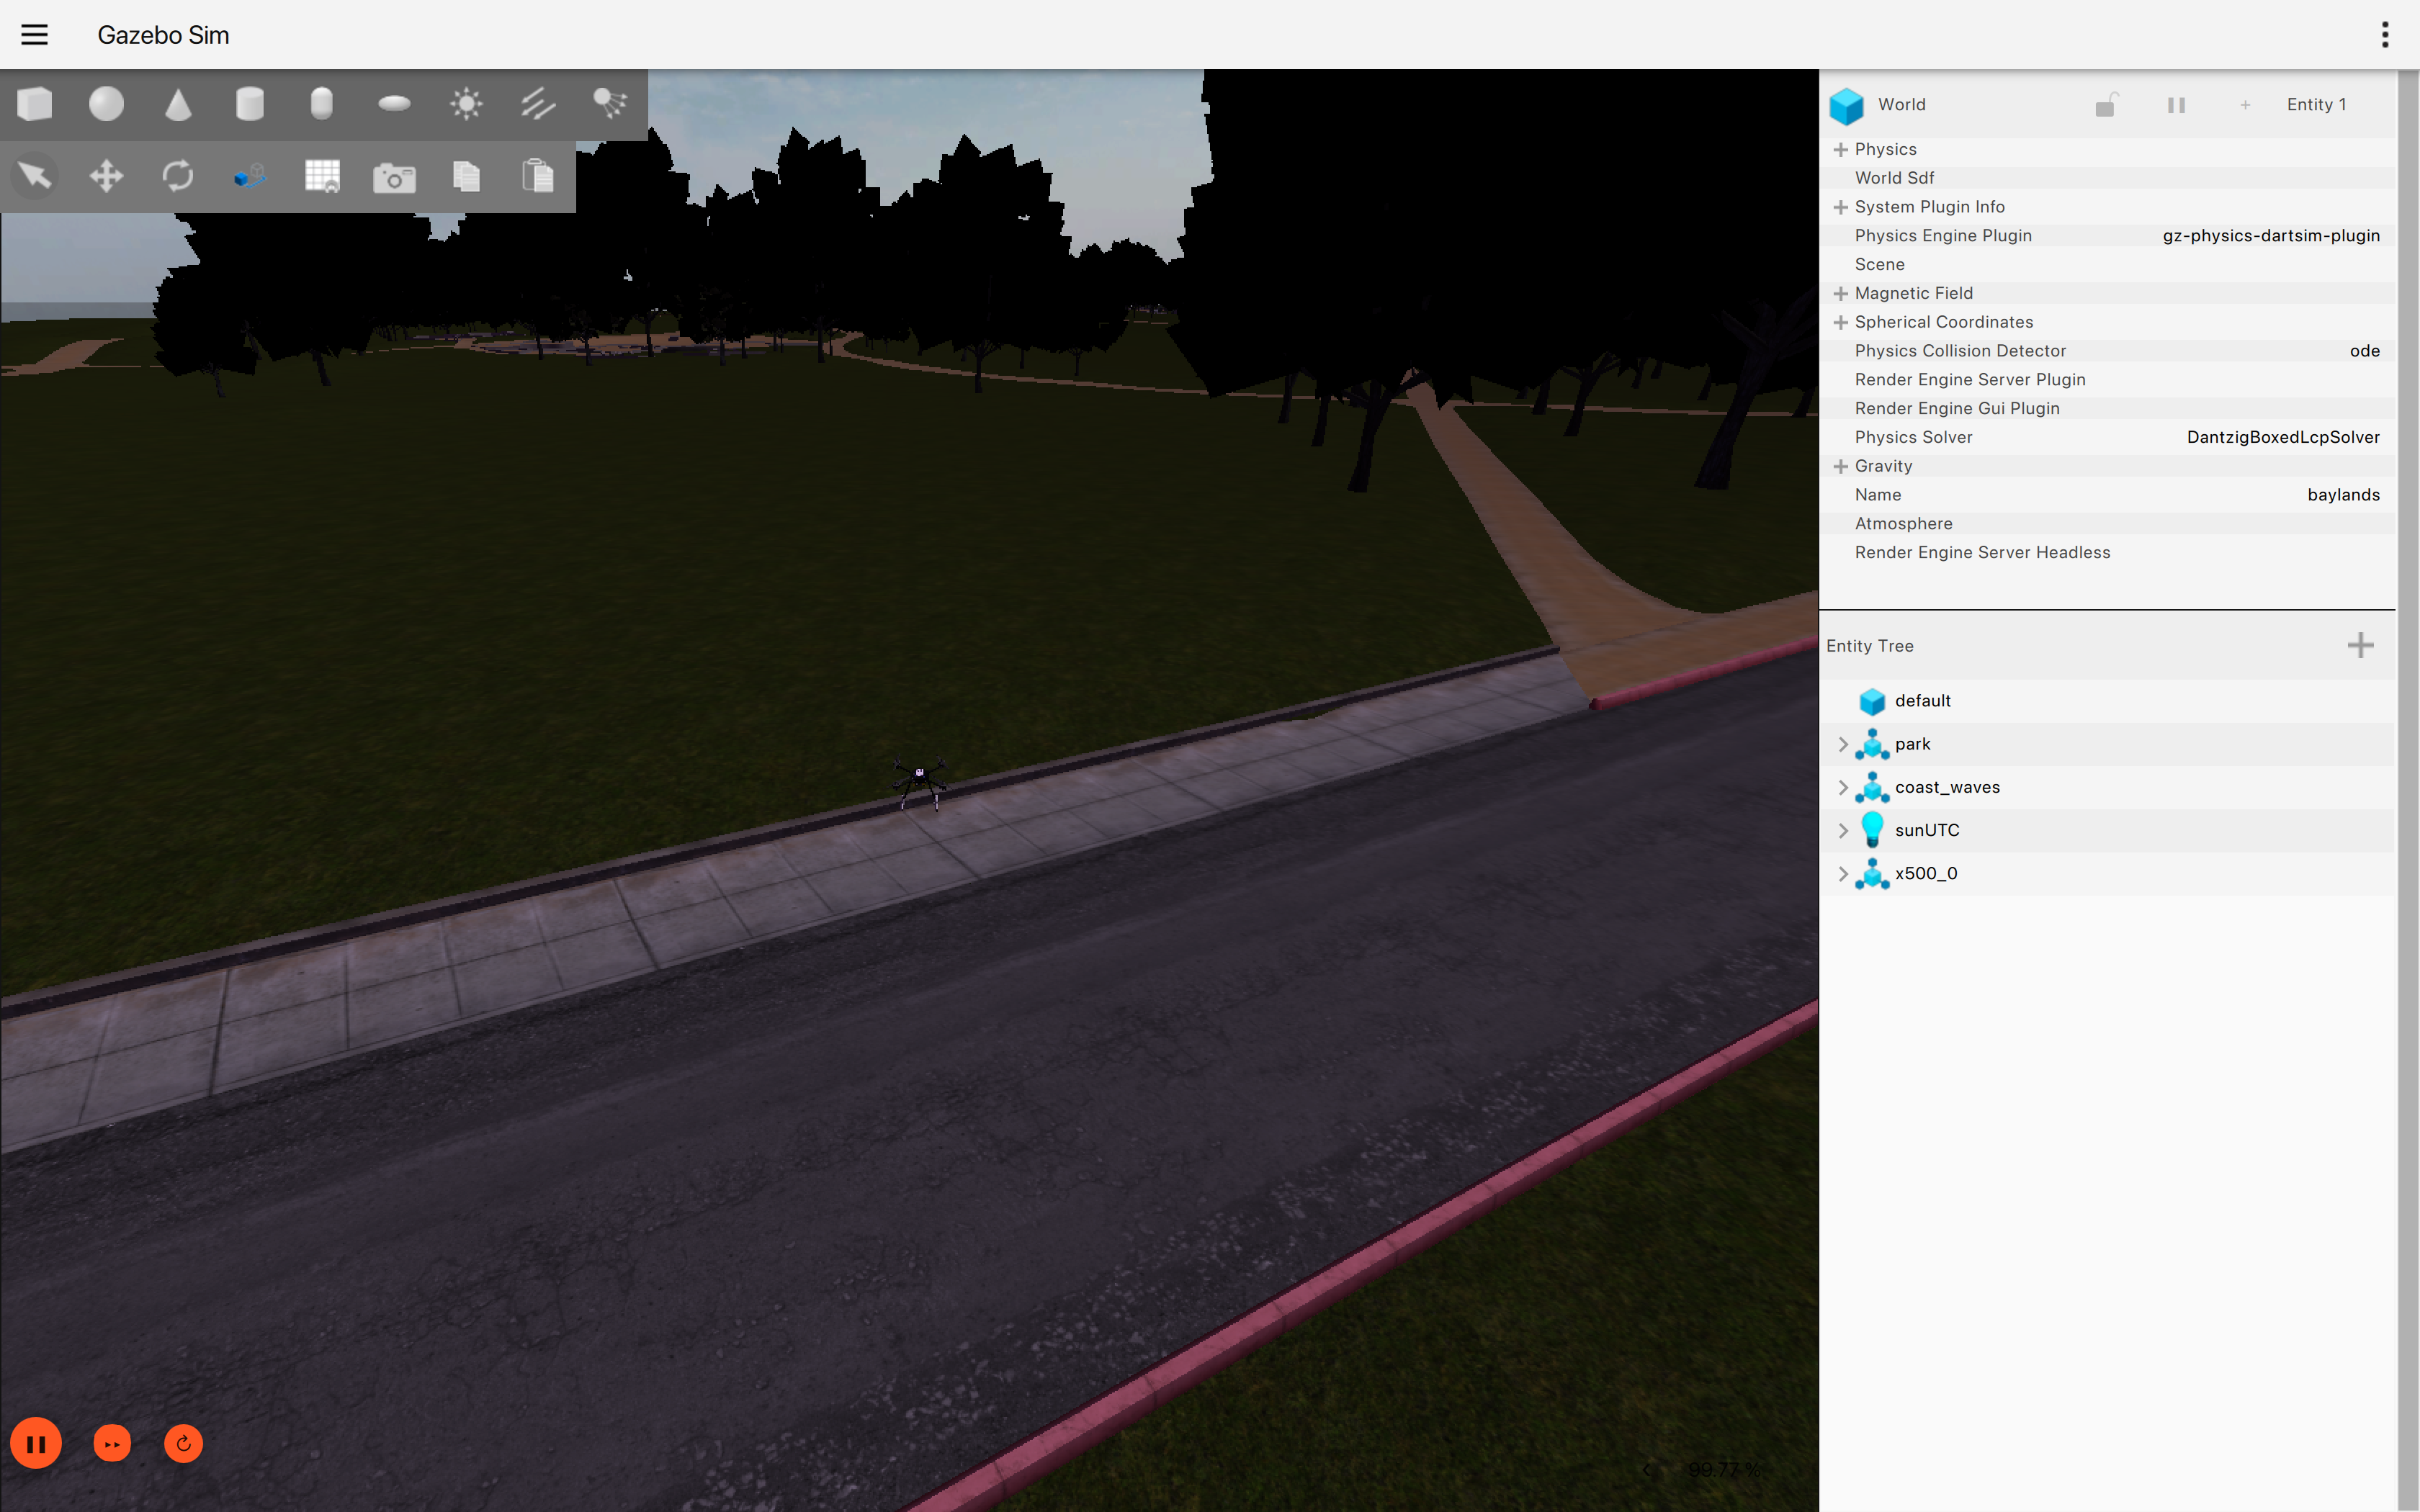
\includegraphics[width=0.7\linewidth]{figures/gazebo_simulation.png}
    \caption{PX4 SITL simulation in Gazebo}
    \label{fig:gazebo}
\end{figure}

The key innovation was the GPS-IMU consistency check, which distinguishes between:
\begin{itemize}
    \item \textbf{Wind/physical disturbance}: Affects both GPS and IMU (body tilts)
    \item \textbf{GPS spoofing}: Affects only GPS; IMU shows no matching motion
\end{itemize}

\begin{table}[htbp]
    \centering
    \caption{8 Heuristic Methods for Auto-Labeling}
    \label{tab:auto_label}
    \begin{tabular}{|l|p{5cm}|p{3cm}|}
        \hline
        \textbf{Method} & \textbf{Description} & \textbf{Threshold} \\
        \hline
        Position Jump & Sudden unrealistic movement >30 m/s & 30.0 m/s \\
        \hline
        Speed Anomaly & Velocity inconsistencies, acceleration >15 m/s$^2$ & 15.0 m/s$^2$ \\
        \hline
        GPS Quality & Low satellites, high eph/epv errors & 6 sats, 5.0m \\
        \hline
        Stale Data & Repeated identical readings $\ge$ 5 cycles & 5 samples \\
        \hline
        Mode Anomaly & Failsafe, unknown mode codes (0x) & - \\
        \hline
        IMU Anomaly & Abnormal angular rates >2 rad/s & 2.0 rad/s \\
        \hline
        Estimator Innovation & Navigation filter inconsistencies & ratios < 0.9 \\
        \hline
        GPS-IMU Consistency & GPS moves without IMU motion (KEY) & IMU < 0.05 rad/s, GPS > 5 m/s \\
        \hline
    \end{tabular}
\end{table}

\subsection{2.3 Feature Engineering for ML Models}

Transforming raw telemetry data into meaningful features for machine learning involved:

\begin{table}[htbp]
    \centering
    \caption{34 Features by Category}
    \label{tab:features}
    \begin{tabular}{|l|p{6cm}|l|}
        \hline
        \textbf{Category} & \textbf{Features} & \textbf{Count} \\
        \hline
        GPS & x\_m, y\_m, alt\_m, rel\_alt\_m, vel\_m\_s, hdg\_deg, fix\_type, satellites\_visible, eph\_m, epv\_m & 10 \\
        \hline
        IMU & roll\_deg, pitch\_deg, yaw\_deg, rollspeed\_radps, pitchspeed\_radps, yawspeed\_radps, vibration\_x/y/z, clipping\_0/1/2 & 12 \\
        \hline
        Estimator & vel\_ratio, pos\_horiz\_ratio, pos\_vert\_ratio, vel\_innov, pos\_horiz\_innov, pos\_vert\_innov & 6 \\
        \hline
        Health & battery\_voltage, battery\_remaining\_pct, armed, failsafe, connection\_ok, is\_stale\_repeat & 6 \\
        \hline
    \end{tabular}
\end{table}

\begin{itemize}
    \item \textbf{Temporal windowing}: 30 samples at 10Hz creates 3-second windows
    \item \textbf{Coordinate transformations}: GPS lat/lon converted to local ENU frame
    \item \textbf{Stride}: 15 samples (50\% overlap) for smooth detection
    \item \textbf{Class distribution}: 37\% anomaly rate (121 anomaly / 327 total windows)
\end{itemize}

\subsection{2.4 System Integration and Management}

We developed a Terminal User Interface (TUI) application using the Rich library that manages:

\begin{itemize}
    \item Start/stop individual components independently
    \item Monitor component status in real-time
    \item Handle process lifecycle (PID management)
    \item Provide access to logs and output
    \item Start All / Stop All batch operations
    \item Train ML models
\end{itemize}

\textbf{TUI Features}:
\begin{itemize}
    \item Interactive component selector with status dashboard
    \item GPS Monitor, Live Inference, Dashboard, PX4 simulation controls
    \item ML Pipeline buttons (Process, Train, Full)
    \item Kill Gazebo for simulation cleanup
    \item Data file information display
\end{itemize}

\subsection{2.5 PX4 Simulation Environment}

We use PX4 Software-in-the-Loop (SITL) simulation with Gazebo for realistic testing:

\begin{itemize}
    \item Full PX4 flight stack execution
    \item Gazebo-based physics simulation (Iris x500 model)
    \item MAVLink communication on UDP port 14560
    \item Interactive pxh shell access
    \item Real-time telemetry output
\end{itemize}